\chapter{Train Tracks}
\label{chap:train tracks}

In this chapter, we introduce the theory of train tracks, which together with the folding automata of Chapter \ref{chap:folding_automata} serve as the primary combinatorial engines for resolving the hyperbolic case of our main result. The ultimate goal of developing this machinery is to rigorously classify the pseudo-Anosov maps that can inhabit the singularity strata identified in Chapter \ref{chap:preliminaries}. By translating the continuous topological dynamics of a surface homeomorphism into a discrete train track map, we can algorithmically constrain its behavior. Specifically, in Chapter \ref{chap:folding_automata} we will construct and utilize train track automata---directed graphs where paths correspond to sequences of valid folding operations---to systematically output the complete, finite list of standard train tracks that must be considered within each stratum.

Historically, the theory of train tracks was originally introduced by Thurston \sidecite{Thurston1988} to study the dynamics of surface homeomorphisms and the classification of mapping classes. This geometric framework was later formalized combinatorially by Penner and Harer \sidecite{penner1992combinatorics}, providing a rigorous calculus for studying laminations on surfaces. Specifically, they formalized the notion of \textit{carrying}, by which they proved that measured laminations can be identified with non-negative weight systems on a train track.

The problem of effectively constructing a train track representative for a given pseudo-Anosov map was subsequently solved by Bestvina and Handel \sidecite{bestvina1995train}. They introduced an algorithm that computes the invariant train track by iteratively folding a graph carried by the surface, a method that serves as the basis for the computational techniques used in this work.

We follow the conventions established by Reinoso \sidecite{reinoso2024pseudo}, who derived them from the work of Song, Ko, and Los \sidecite{SongEntropy} and Ham and Song \sidecite{HamSong2007}.

\section{Train Tracks on a Compact Surface}

Let $S$ be a compact surface, possibly with non-empty boundary, and containing a set $Q$ of $n$ marked points. We first provide the general topological definition of a train track on $S$.

\begin{definition}[Train Track]\label{def:train_track_general}
    A \textit{train track} on $S$ is a smooth, branched 1-submanifold $\tau \subset S$ satisfying the following conditions:
    \begin{enumerate}
        \item $\tau$ is contained in the interior $S \setminus \partial S$.
        \item The branch points of $\tau$, referred to as \textit{switches}, have valence at least $3$.
        \item \textbf{Tangency:} At every switch $v$, the tangent vectors of the incident branches are collinear. Consequently, there is a well-defined tangent line $T_v \tau$ in the tangent space $T_v S$.
        \item \textbf{Cusps:} If two branches incident to a switch $v$ share the same ray of the tangent line (i.e., their tangent vectors point in the same direction), we say they form a \textit{cusp}.
        \item \textbf{Complementary Regions:} Every component of the complement $S \setminus \tau$ is either an unpunctured polygon with $k \geq 3$ sides or a once-punctured polygon with $k \geq 1$ sides (where ``sides'' are branches of $\tau$ and ``vertices'' are switches).
    \end{enumerate}
\end{definition}

We consider two train tracks $\tau_1$ and $\tau_2$ to be \textbf{equivalent} if they are smoothly isotopic relative to the marked points $Q$. Formally, there exists a smooth family of embeddings $h_t: \tau \to S$ for $t \in [0,1]$ such that $h_0(\tau) = \tau_1$, $h_1(\tau) = \tau_2$, and for all $t$, $h_t(\tau)$ is a valid train track disjoint from $Q$. From this point on, unless otherwise stated, we speak of train tracks on a surface up to equivalency.

\subsection{The Underlying Graph}
It will be necessary to separately consider certain combinatorial data of a train track from its smooth embedding.

\begin{definition}[Underlying Graph]
    The \textit{underlying graph} of a train track $\tau$, denoted $G_\tau$, is the 1-dimensional CW-complex obtained by forgetting the $C^1$ tangency structure at the switches.
    \begin{itemize}
        \item The vertex set $V(G_\tau)$ consists of the switches of $\tau$.
        \item The edge set $E(G_\tau)$ consists of the branches of $\tau$.
    \end{itemize}
    Two train tracks $\tau_1$ and $\tau_2$ have isomorphic underlying graphs if there is a graph isomorphism $\varphi: G_{\tau_1} \to G_{\tau_2}$.
\end{definition}

\begin{remark}
    An isomorphism of underlying graphs does not imply the train tracks are equivalent, as the graph $G_\tau$ itself does not encode the embedding information into the surface $S$. In the terminology of \cite{SongEntropy}, the graph $G_\tau$ corresponds to the \textit{skeleton}, while the train track $\tau$ constitutes a specific \textit{marking} (embedding) of that skeleton which encodes the cusp data.
\end{remark}

\begin{figure}[h]
    \centering
    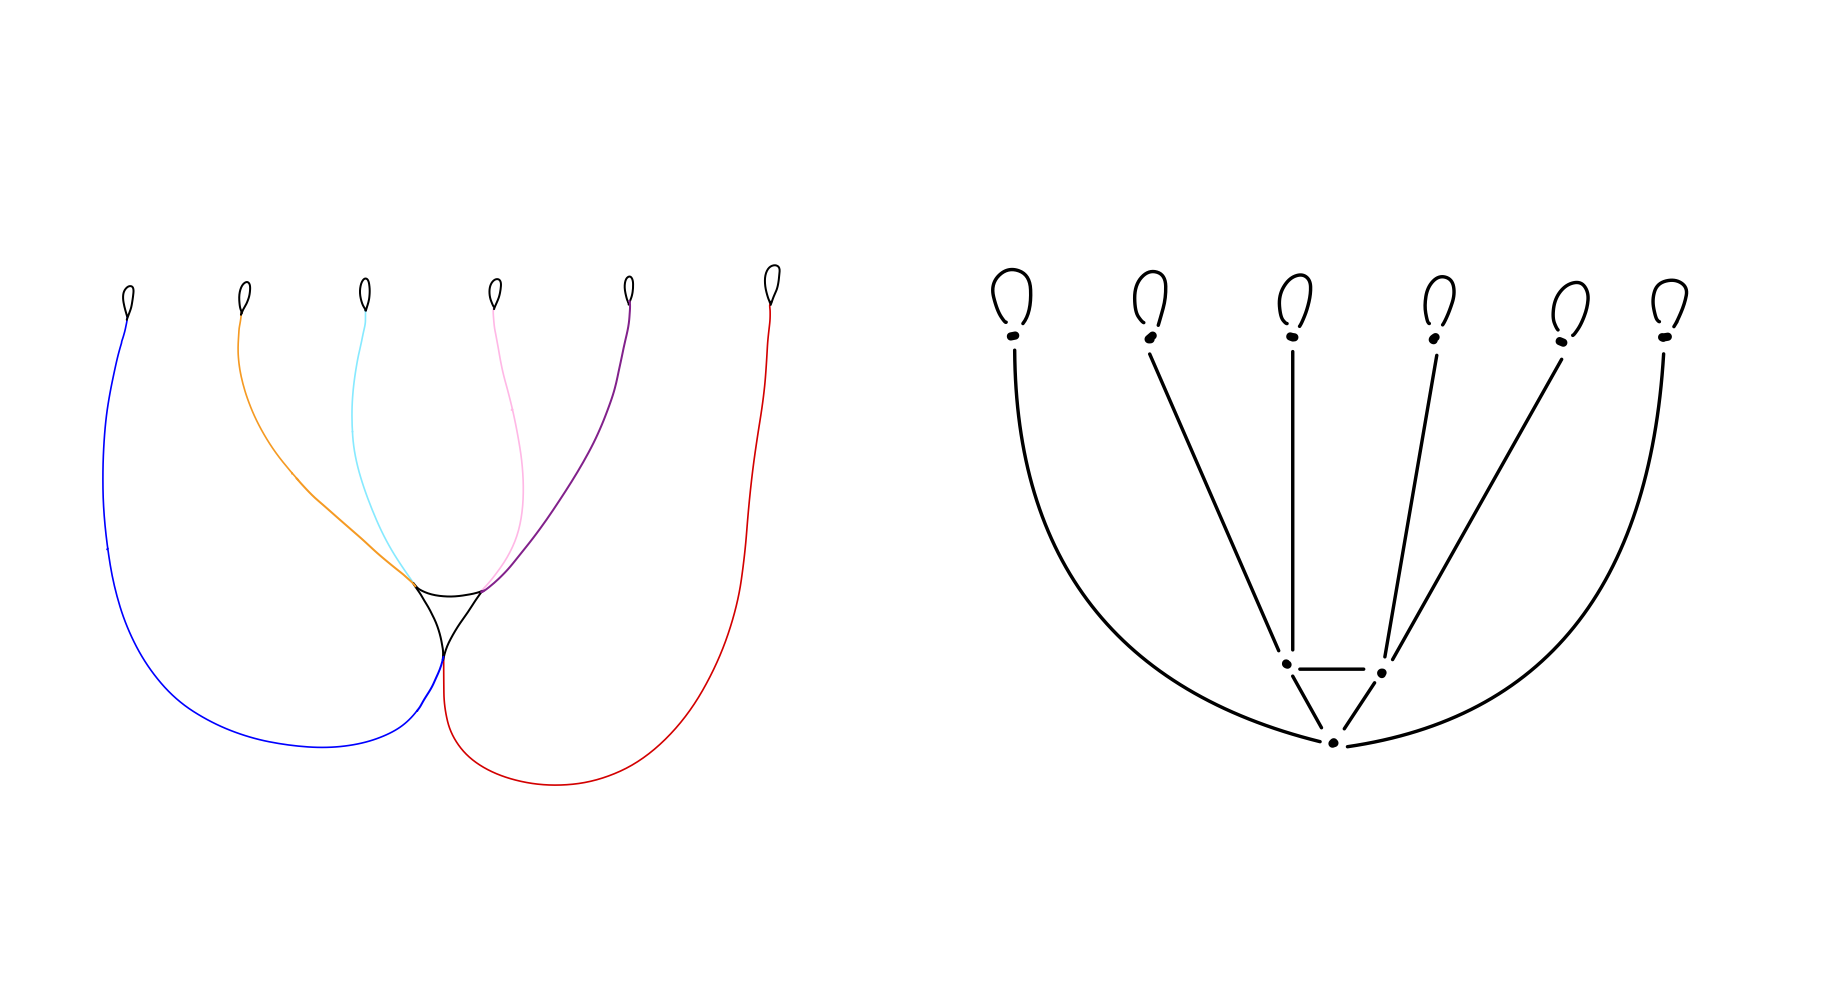
\includegraphics[width=0.8\linewidth]{figures/traintrack_underlying_graph.png}
    \caption{A train track and its underlying graph.}
    \label{fig:traintrack_underlying_graph}
\end{figure}

\section{Train Track Maps and Dynamics}
\label{sec:traintrack_maps}

Having established the geometric structure of train tracks, we now define the notion of carrying and the dynamics of maps on the track. We follow the definitions provided in Reinoso \cite[Section 2.2]{reinoso2024pseudo}.

\subsection{Carrying and Fibered Neighborhoods}
To relate train tracks to surface homeomorphisms formally, we use the notion of a fibered neighborhood.

\begin{definition}[Fibered Neighborhood]
    A \textit{fibered neighborhood} $F(\tau) \subset S$ is a tubular neighborhood of the train track $\tau$ equipped with a singular foliation by vertical fibers. The leaves of this foliation are transverse to the branches of $\tau$ and are singular only at the switches (corresponding to the corners of the polygonal complementary regions).
\end{definition}

Now we are ready to define what it means for a train track to ``carry'' a surface homeomorphism.

\begin{definition}[Carrying]
    A homeomorphism $\phi_h: S \to S$ is said to be \textit{carried} by $\tau$ if $\phi_h(\tau)$ can be isotoped into the interior of $F(\tau)$ such that the image is everywhere transverse to the vertical fibers.

    We say that a mapping class $h \in \mathrm{Mod}(S)$ is carried by $\tau$ if its geometric representative $\phi_h$ is carried by $\tau$.
\end{definition}

\begin{figure}[h]
    \centering
    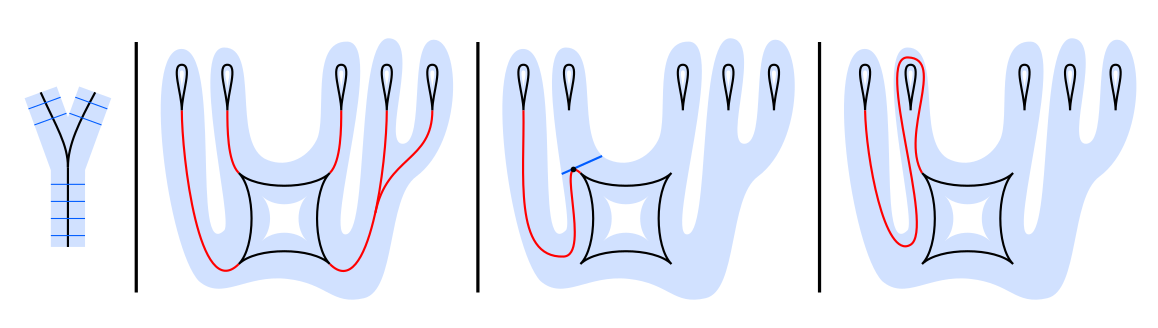
\includegraphics[width=0.8\linewidth]{figures/traintrack_neighborhood.png}
    \caption{A fibered neighborhood $F(\tau)$ of a train track $\tau$, with vertical fibers shown transverse to the branches.}
    \label{fig:fibered_neighborhood}
\end{figure}

\subsection{Train Paths and Maps}
When $\phi_h$ is carried by $\tau$, we can project the image $\phi_h(\tau)$ along the fibers of $F(\tau)$ back onto $\tau$. This projection induces a combinatorial map on the track itself. To make this more precise, we make use of the following definitions:

\begin{definition}[Train Path]
    A \textit{train path} on $\tau$ is a smooth immersion $\gamma: [0,1] \to \tau$ mapping endpoints to switches. Crucially, $\gamma$ must respect the tangent structure: it may pass through a switch smoothly, but it may not turn back at a cusp (i.e., it cannot backtrack against the flow).
\end{definition}

\begin{definition}[Train Track Map]
    A \textit{train track map} is a continuous surjection $f: \tau \to \tau$ such that:
    \begin{enumerate}
        \item $f$ maps switches to switches.
        \item For any train path $\gamma$, the composition $f \circ \gamma$ is a valid train path.
    \end{enumerate}
\end{definition}

This definition ensures that the map $f$ does not ``fold'' the track back onto itself arbitrarily; it preserves the smooth directionality of the branches.

When $\phi_h$ is carried by a train track $\tau$, there is naturally an induced train track map $f_h \colon \tau \to \tau$, determined by the image $\phi_h(\tau)$ under $\phi_h$. For an edge $e$ of $\tau$, we define $f_h(e)$ to be the train path that the image $\phi_h(e) \subset F(\tau)$ collapses onto under the natural deformation retraction $F(\tau) \to \tau$.

Figure \ref{fig:traintrack_map} shows an example of an illustration of a train track map. On the left is a train track $\tau$, where we have named seven of the edges: $b,o,s,i,p,r$ and given them (arbitrary) orientations, all oriented toward the monogons. The image of each of these colored edges is the following:
\[
\fbb = s
\]
\[
\fbo = i
\]
\[
\fbs = p r
\]
\[
\fbi = bo
\]
\[
\fbp = b
\]
\[
\fbr = o b p
\]

The image of the black edges making up the polygons can be inferred from the image of the above edges.

\begin{figure}
    \centering
    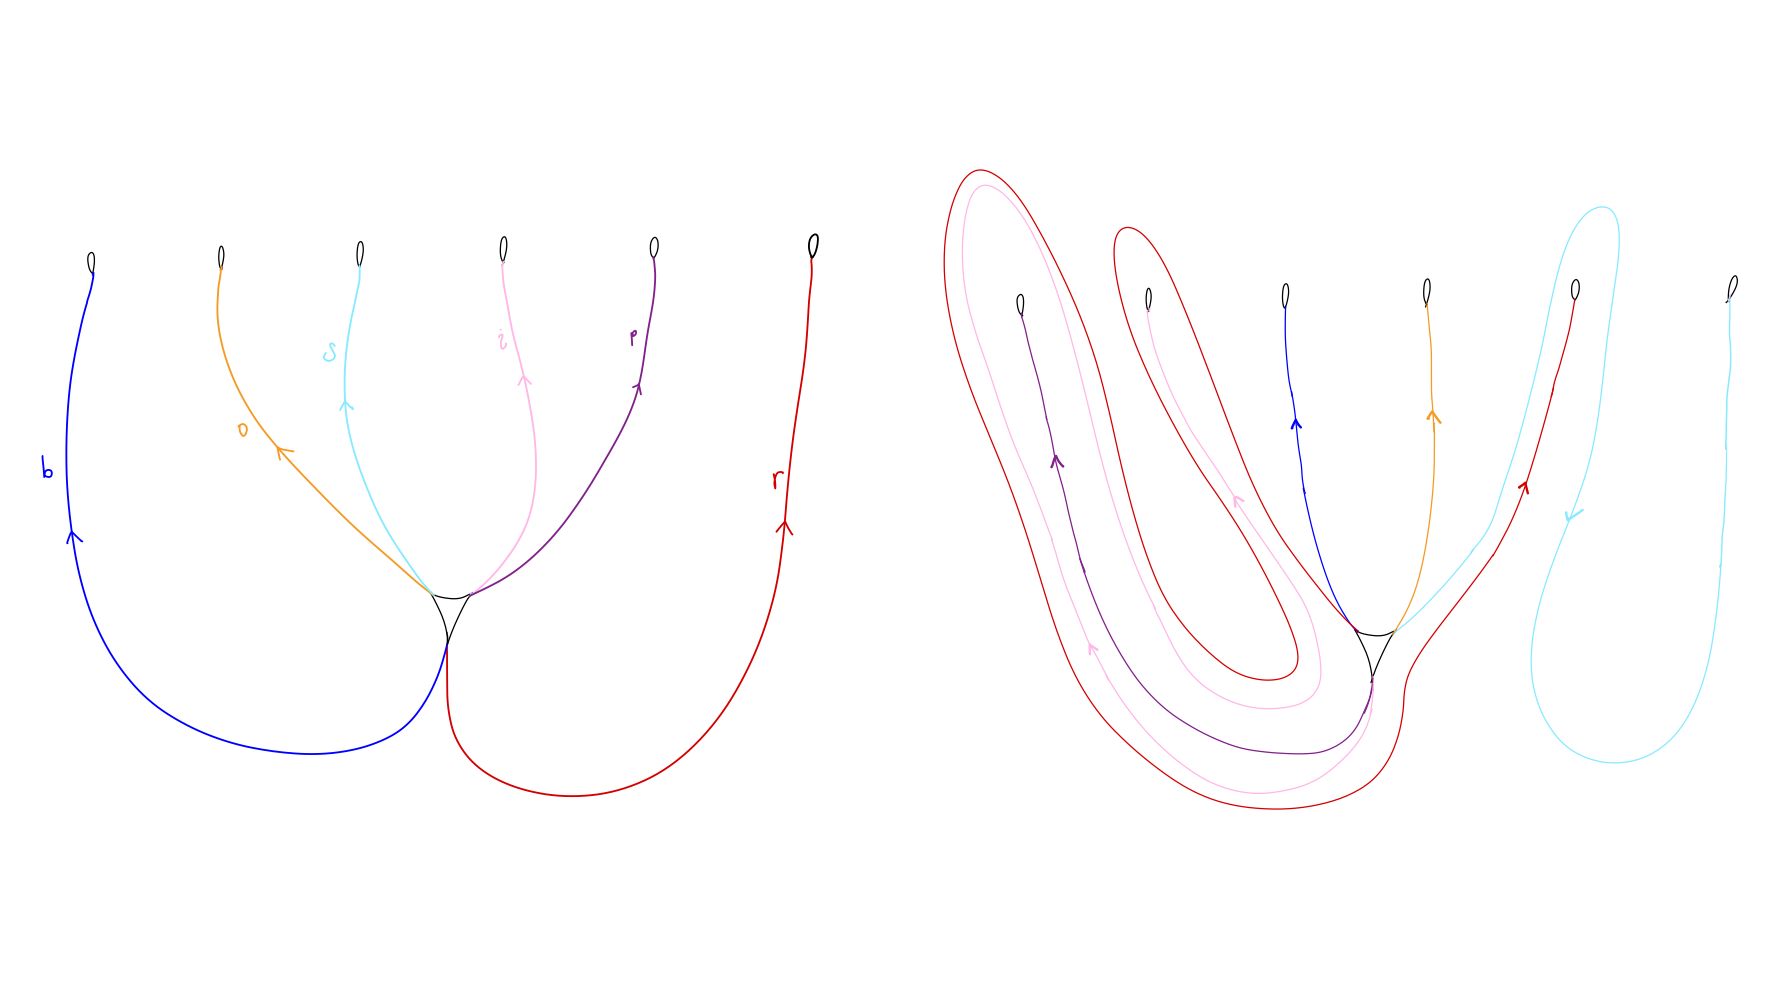
\includegraphics[width = \linewidth]{figures/traintrack_map.png}
    \caption{Left: A train track $\tau$. Right: A train track map $f \colon \tau \to \tau$.}
    \label{fig:traintrack_map}
\end{figure}

An important result of Bestvina-Handel is the fact that a geometric representative $\phi_h$ of a mapping class $h \in \mathrm{Mod}(S)$ is completely determined by its induced train track map on a train track that carries $\phi_h$:

\begin{theorem}[{\cite{bestvina1995train}, \cite[Theorem~2.2.1]{reinoso2024pseudo}}] \label{theorem:bestvina-handel mapping class determined by train track map}
Let $h, g \in \mathrm{Mod}(S)$ be two mapping classes with geometric representatives $\phi_h, \phi_g$, respectively. Suppose that $h$ and $g$ are carried by the same train track $\tau$, and induce maps $f_h, f_g \colon \tau \to \tau$. If $f_h = f_g$, then $h$ and $g$ are freely isotopic and $\phi_h = \phi_g$.
\end{theorem}

Applying Theorem \ref{theorem:bestvina-handel mapping class determined by train track map} to the specific case of maps on the $n$-marked disk, we have the following corollary:

\begin{corollary}[{\cite[Corollary~2.2.2]{reinoso2024pseudo}}]\label{cor:induce_by_braid_fulltwist}
    Let $\alpha, \beta \in \mathrm{Mod}(D_n)$ be two $n$-braids which are carried by the same track $\tau$ and induce the same train track map $f_\alpha = f_\beta \colon \tau \to \tau$. Then, we have
    \[
    \phi_\alpha = \phi_\beta,
    \]
    and
    \[
    \alpha = \Delta^{2k} \beta
    \]
    for some $k \in \mathbb{Z}$, where $\Delta^2 = (\sigma_1 \dots \sigma_{n - 1})^n$ is a full twist about $\partial D_n$.
\end{corollary}

Corollary \ref{cor:induce_by_braid_fulltwist} resolves the full-twist ambiguity in the Birman-Hilden disk braid noted in Remark \ref{rem:fulltwist_ambiguity}. The disk braid $\beta \in \mathrm{Mod}(D_6)$ associated to a hyperbolic fibered knot $K$ via the Birman-Hilden correspondence is well-defined only up to powers of $\Delta_6^2$. By the corollary, two braids carried by the same train track and inducing the same train-track map differ exactly by a power of $\Delta_6^2$. The train-track framework therefore captures each disk braid at precisely the resolution at which it is canonically defined: a coset of $\langle \Delta_6^2 \rangle$ in $\mathrm{Mod}(D_6)$, represented by a unique train-track map. All downstream obstructions in this dissertation --- the orientability obstruction of Chapter \ref{chap:stratoriented}, the homological filter of Chapter \ref{chap:stratatraintrackanalysis}, and the trace and absorption obstructions of Chapter \ref{chap:stratatraintrackanalysis} --- depend on the disk braid only through its train-track signature, and therefore factor through the quotient $\mathrm{Mod}(D_6)/\langle \Delta_6^2 \rangle$ automatically.

We formalize the relationship between a mapping class and its combinatorial representation through the concept of \textit{geometric data}. For a mapping class $h \in \mathrm{Mod}(S)$, the geometric data is defined as the tuple
\[
(h, \phi_h, \tau, f_h),
\]
comprising the mapping class $h$, its geometric representative $\phi_h$, a train track $\tau$ that carries $h$, and the induced train track map $f_h: \tau \to \tau$.

While a single mapping class may be carried by a variety of distinct train tracks, the induced map $f_h$ is uniquely determined by the choice of $\tau$. It is important to distinguish this structure from general train tracks; an arbitrary train track does not necessarily carry a mapping class, nor does every train track map on a track correspond to a surface homeomorphism. However, when this data exists---particularly in the pseudo-Anosov case---the train track $\tau$ effectively encodes the geometry of the mapping class, as the following proposition shows:

\begin{prop}[{\cite{bestvina1995train}}] \label{prop:B-H train track polygon enclosure}
Let $h$ be a pseudo-Anosov mapping class carried by $\tau$. If $N$ is a connected interior (resp. peripheral) component of $S \setminus \tau$, then $\tau$ has $p$ cusps along $\partial N$ if and only if $\phi_h$ has a $p$-pronged singularity in the interior of $N$ (resp. a $p$-pronged boundary in $N$).
\end{prop}

\begin{remark}[Terminology in the literature]
    We note that in the broader literature on surface dynamics (e.g., Penner-Harer \cite{penner1992combinatorics}, Bestvina-Handel \cite{bestvina1995train}), a train track $\tau$ satisfying the condition that $f_h(\tau)$ is carried by $\tau$ in an efficient manner (specifically, with a non-negative transition matrix) is typically referred to as an \textit{invariant train track}.

    In this work, we follow the conventions of Reinoso \cite{reinoso2024pseudo}, where this invariance property is intrinsic to the definition of \textit{geometric data} for a pseudo-Anosov mapping class. Consequently, we will generally avoid the term ``invariant train track'' and instead refer to the tuple $(h, \phi_h, \tau, f_h)$ as the geometric data associated with the map.
\end{remark}


\section{Relationship to Invariant Foliations}
\label{sec:train track and foliations}

The utility of train tracks in studying pseudo-Anosov homeomorphisms arises from their relationship with the invariant measured foliations. Recall from the definition of a pseudo-Anosov map $\phi \colon \Sigma \to \Sigma$, that it preserves a pair of transverse measured singular foliations: the unstable foliation $\mathcal{F}^u$ (which is expanded by a factor $\lambda > 1$) and the stable foliation $\mathcal{F}^s$ (which is contracted by $1/\lambda$).

Following Thurston \sidecite{Thurston1988} and the formalization by Penner and Harer \sidecite{penner1992combinatorics}, a train track $\tau$ carrying a pseudo-Anosov $\phi$ can be understood as a $C^1$ \textit{smoothing} of the singular foliation $\mathcal{F}^u$. This creates a correspondence between the invariant foliations of a pseudo-Anosov $\phi_h$ and a train track that carries it. This is made explicit in the construction of Bestvina and Handel \sidecite{bestvina1995train} (also see Reinoso \sidecite{reinoso2024pseudo}), and is rigorous in the following sense:

The algorithm developed by Bestvina and Handel provides a systematic method for constructing a train track $\tau$ that carries a pseudo-Anosov homeomorphism $\phi_h$. Central to this construction is the concept of an \emph{efficient fibered surface} $F \subset S$, which acts as a deformation retract of the surface $S$. The surface $F$ admits a decomposition into rectangular \emph{strips} and disk-like \emph{junctions}, where the strips connect the junctions and are foliated by arcs parallel to the junction boundaries.

To pass from this fibered surface to the train track $\tau$, one performs a controlled collapse of the decomposition. While the strips collapse to form the \emph{real edges} of the track, the junctions are not merely collapsed to vertices; rather, they are refined into a complex of \emph{infinitesimal edges} determined by the local dynamics of $\phi_h$. This structure ensures that the induced train track map $f_h: \tau \to \tau$ restricts to an automorphism on the subgraph of infinitesimal edges. Consequently, the topological characteristics of the complementary regions within the junctions---referred to as \emph{infinitesimal polygons}---are preserved. Specifically, $f_h$ maps any infinitesimal polygon to an image with an identical number of cusps.

On the other hand, given a train track $\tau$ that carries $\phi_h$, one can recover the invariant foliations (up to isotopy), so that $\tau$ lies tangent to $\mathcal{F}^u$ and transverse to $\mathcal{F}^s$. By Proposition \ref{prop:B-H train track polygon enclosure}, each connected interior/peripheral region is a $k$-sided polygon, with a $k$-pronged singularity within. In this way, there exists an embedding of the unstable foliation $\mathcal{F}^u$ into the fibered neighborhood $N(\tau)$. Under this embedding, every regular leaf of $\mathcal{F}^u$ is everywhere transverse to the vertical fibers of $N(\tau)$. Consequently, the branches of $\tau$ are isotopic to the leaves of $\mathcal{F}^u$ away from the singularities. See Figure \ref{fig:foliation_models}.

\begin{figure}
    \centering
    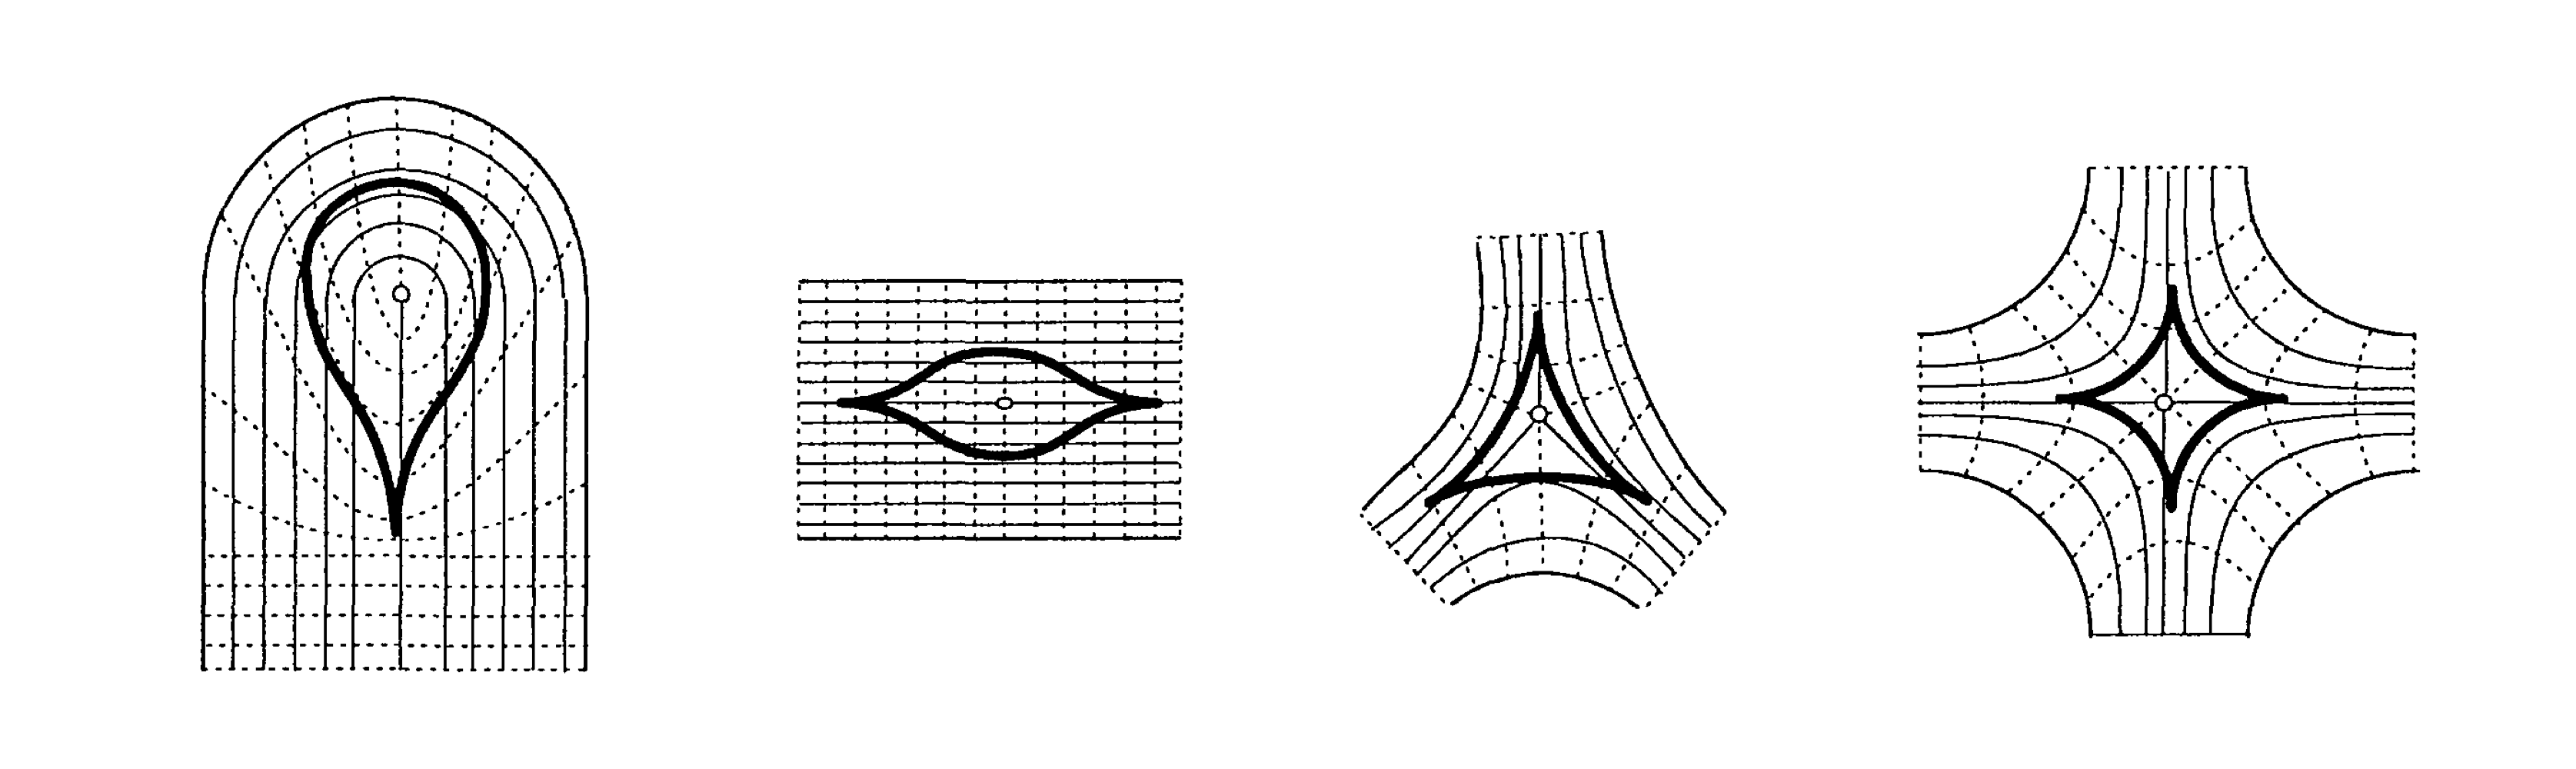
\includegraphics[width=\linewidth]{figures/foliations_track.png}
    \caption[Local models of $k$-pronged singularities]{Local models of $k$-pronged singularities ($k=1, 2, 3, 4$). The solid lines, tangent to the boundaries of the central complementary regions, represent the leaves of the unstable foliation $\mathcal{F}^u$. The transverse dotted lines represent the leaves of the stable foliation $\mathcal{F}^s$.}
    \label{fig:foliation_models}
\end{figure}

\section{Real and Infinitesimal Edges}
Since the details of the Bestvina-Handel construction are not of central importance to our work, it suffices for us to take the following equivalent notion of \emph{infinitesimal edges} and \emph{real edges}. For us, it is merely a matter of combinatorial convenience in distinguishing those edges of a train track that enclose an interior singularity to form polygons, from those edges which connect these polygons.

\begin{itemize}
    \item \textbf{Infinitesimal Edges ($E_{\text{inf}}$):} Edges that lie on the boundary of the connected regions of $S\setminus \tau$ containing the marked points and interior non-marked singularities. In the context of the invariant foliation, these correspond to the separatrices near these singularities and carry zero transverse measure. We refer to the polygons they make up as \emph{marked/unmarked infinitesimal polygons}, depending on whether they enclose a marked point or a non-marked interior singularity.
    \item \textbf{Real Edges ($E_{\text{real}}$):} All edges of $\tau$ not in $E_{\text{inf}}$. These edges connect the infinitesimal regions and carry the dynamics of the map.\footnote{Ham and Song \cite{HamSong2007} refer to these as ``expanding edges,'' a term highlighting their role in the Markov partition. We retain Reinoso's terminology for consistency.}
\end{itemize}

% FIGURE PLACEHOLDER

\subsection*{The Transition Matrix}
Using the terminology of real and infinitesimal edges, we can define the \emph{transition matrix} of a train track map, in which the combinatorial dynamics are encoded. Since the infinitesimal edges carry zero measure, they are ignored in dynamical calculations and so their image under the train track map does not appear in the matrix. For full details, see the work of Bestvina-Handel \sidecite{bestvina1995train}.

\begin{definition}[Transition Matrix]
    Let $E_{\text{real}}(\tau) = \{e_1, \dots, e_m\}$ be the set of \textit{real edges} of a train track $\tau$. The \textit{transition matrix} $M(f_h)$ is the $m \times m$ non-negative integer matrix where the entry $M_{ij}$ records the number of times the image $f_h(e_j)$ traverses the edge $e_i$ in either direction.
\end{definition}

\begin{theorem}[Perron-Frobenius \cite{bestvina1995train, reinoso2024pseudo}]
    Let $h$ be a pseudo-Anosov mapping class carried by $\tau$, with geometric representative $\phi_h$, inducing the train track map $f_h: \tau \to \tau$. Then the transition matrix $M(f_h)$ is a Perron-Frobenius matrix. The spectral radius of $M(f_h)$ is exactly the dilatation $\lambda(\phi_h)$ of the pseudo-Anosov map. In this case, the dilatation $\lambda (\phi_h )$ is the largest eigenvalue of $M(f_h)$, and the number of fixed points of $\phi_h$ is bounded in terms of the trace of $M(f_h)$:
    \[
    \mathrm{tr}(M(f_h)) \leq \abs{\mathrm{Fix}(\phi_h)}.
    \]
\end{theorem}

\section{Standard Train Tracks on the Marked Disk}
\label{sec:standard_tracks}

We now restrict our attention to the unit disk $D_n$ with $n$ marked points $Q = \{q_1, \dots, q_n\}$. We utilize the subclass of \emph{standard train tracks} defined by Ko-Los-Song \sidecite{SongEntropy}, Farber-Reinoso-Wang \sidecite{farber2024fixed}, and Reinoso \sidecite{reinoso2024pseudo}. A result of Ko-Los-Song ensures that every pseudo-Anosov map on $D_n$ is carried by such a track.

\begin{definition}[Standard Train Track]\label{def:standard_track}
    A train track $\tau \subset D_n$ is \textit{standard} if:
    \begin{enumerate}
        \item \textbf{Infinitesimal Polygons:} Every component of $D_n \setminus \tau$ disjoint from $\partial D_n$ is an \textit{infinitesimal polygon}. Its boundary consists entirely of infinitesimal edges.
        \item \textbf{Switches:} The set of switches coincides with the vertices of these infinitesimal polygons.
        \item \textbf{Tangency Structure:}
        \begin{itemize}
            \item Two adjacent infinitesimal edges at a switch share a common tangent (forming a smooth boundary for the polygon).
            \item Two adjacent real edges at a switch share a common tangent.
            \item A real edge and an infinitesimal edge at a switch are never tangent; they meet at a cusp.
        \end{itemize}
        \item \textbf{Vertical Marking:} For each marked point $q_i$, there is exactly one infinitesimal edge of $\tau$ passing vertically above $q_i$. No other edge intersects the vertical ray extending upwards from $q_i$.
    \end{enumerate}
\end{definition}

Condition 4 is essential for identifying the mapping class group of the punctured disk with the braid group $B_n$. It ensures the track is ``pinned'' in a canonical way relative to the standard braid generator positions.

\begin{prop}[{\cite{SongEntropy}}]\label{prop:every_pA_carried_by_standard_track}
    Every pseudo-Anosov map on a marked disk is carried by a standard train track.
\end{prop}

\section{Jointless Train Tracks}
\label{sec:jointless_tracks}

While Proposition \ref{prop:every_pA_carried_by_standard_track} ensures that every pseudo-Anosov map on the disk is carried by a standard train track, this carrying track is not strictly unique. To obtain a canonical representative---and specifically one that facilitates the algorithmic detection of fixed points---we can restrict our attention to a well-behaved subclass of standard tracks by eliminating localized regions of combinatorial complexity known as \textit{joints}.

\begin{definition}[Joint]
\label{def:joint}
    Let $\tau$ be a standard train track. A \textit{joint} is a switch $v$ located on an infinitesimal monogon (a region surrounding a single marked point) such that $v$ is incident to at least two real edges.
\end{definition}

Reinoso \sidecite{reinoso2024pseudo} showed that for a broad class of pseudo-Anosov maps, these joints can be systematically eliminated through a graph-refinement operation known as \textit{tight splitting}.

The formal mechanics of tight splitting will be rigorously defined and utilized in Chapter \ref{chap:tight_splitting} to systematically reduce the list of train tracks to consider. For the purposes of our foundational setup, it suffices to rely on the following guarantee by Reinoso, which assures us that tight splitting will always successfully yield a jointless representative for the maps we care about:

\begin{theorem}[{\cite[Theorem~C]{reinoso2024pseudo}}]\label{theorem:theorem C jointless}
Let $\phi_\beta$ be a pseudo-Anosov representative of a braid $\beta$ on the marked disk. Assume that the invariant foliations of $\phi_\beta$ have at least one $k$-pronged singularity away from the boundary with $k \geq 2$. Then, $\phi_\beta$ is carried by a standard train track $\tau$ with no joints.
\end{theorem}

\begin{corollary}[{\cite[Corollary~6.2.9]{reinoso2024pseudo}}]
\label{cor:jointless_track}
    Let $\phi_\beta$ be a pseudo-Anosov homeomorphism on the $n$-punctured disk $D_n$. Suppose that the invariant foliations of $\phi_\beta$ have at least one $k$-pronged singularity in the interior of $D_n$ (away from the boundary) with $k \geq 2$. Then $\phi_\beta$ is carried by a standard train track $\tau$ that has no joints.
\end{corollary}

Because the monodromy of our hypothetical genus-two knot necessarily involves $3$-pronged or $4$-pronged interior singularities (as classified in Table \ref{tab:prong_configurations}), we safely satisfy the hypothesis of Corollary \ref{cor:jointless_track}. Consequently, we may strictly restrict our attention to jointless standard train tracks moving forward. In such tracks, every marked point is enclosed by a monogon incident to exactly one real edge, or is part of a larger polygon.

\section{Lifting Train Track Maps}
\label{sec:lifting train tracks}

To bridge the gap between the combinatorial dynamics of braids on the disk and the topology of genus-two knots in 3-manifolds, we consider the Birman-Hilden correspondence as described in Section \ref{section:Birman-Hilden} (with the surface conventions of Section \ref{sec:notation}). Under this correspondence, train tracks, as well as their associated maps on the disk, can be lifted back to the genus-two surface.

\subsection{Geometric Lifting of Standard Tracks}
To analyze the fixed-point properties of the surface map $\phi_\Phi \colon \Sigma_2^2 \to \Sigma_2^2$, we lift standard train tracks from the disk to the surface $\Sigma_2^2$ via the branched double covering map $\pi$. Let $\tau \subset D^2$ be a standard train track carrying the pseudo-Anosov braid $\beta$. Since $\tau$ is embedded in $D^2$, its full preimage $\tilde{\tau} = \pi^{-1}(\tau)$ yields a graph embedded in $\Sigma_2^2$ which is inherently invariant under the hyperelliptic involution $\iota$.

The geometric construction of the lifted track $\tilde{\tau}$ is strictly dictated by the local behavior of the covering map, which we illustrate in Figure \ref{fig:reinoso_lift_visual}. The components lift as follows:
\begin{enumerate}
    \item \textbf{Real Edges:} Each real edge of $\tau$ avoids the branch points and therefore lifts to two distinct real edges in $\tilde{\tau}$, which are interchanged by $\iota$.
    \item \textbf{Interior Singularities:} An infinitesimal polygon with $k$ sides in the interior of $D^2$ (away from the marked points) lies in the unbranched region of the cover. It therefore lifts to a pair of disjoint $k$-sided polygons in $\tilde{\tau}$, swapped by $\iota$.
    \item \textbf{Boundary Behavior:} The boundary of the disk $\partial D^2$ lifts to the two boundary components of $\Sigma_2^2$, denoted $\partial_z$ and $\partial_p$, which are swapped by $\iota$. An infinitesimal $k$-gon adjacent to $\partial D^2$ lifts to a $2k$-gon bounding $\partial_z$ and a $2k$-gon bounding $\partial_p$, reflecting the local doubling of the cone angle.
\end{enumerate}

\begin{figure}[ht]
    \centering
    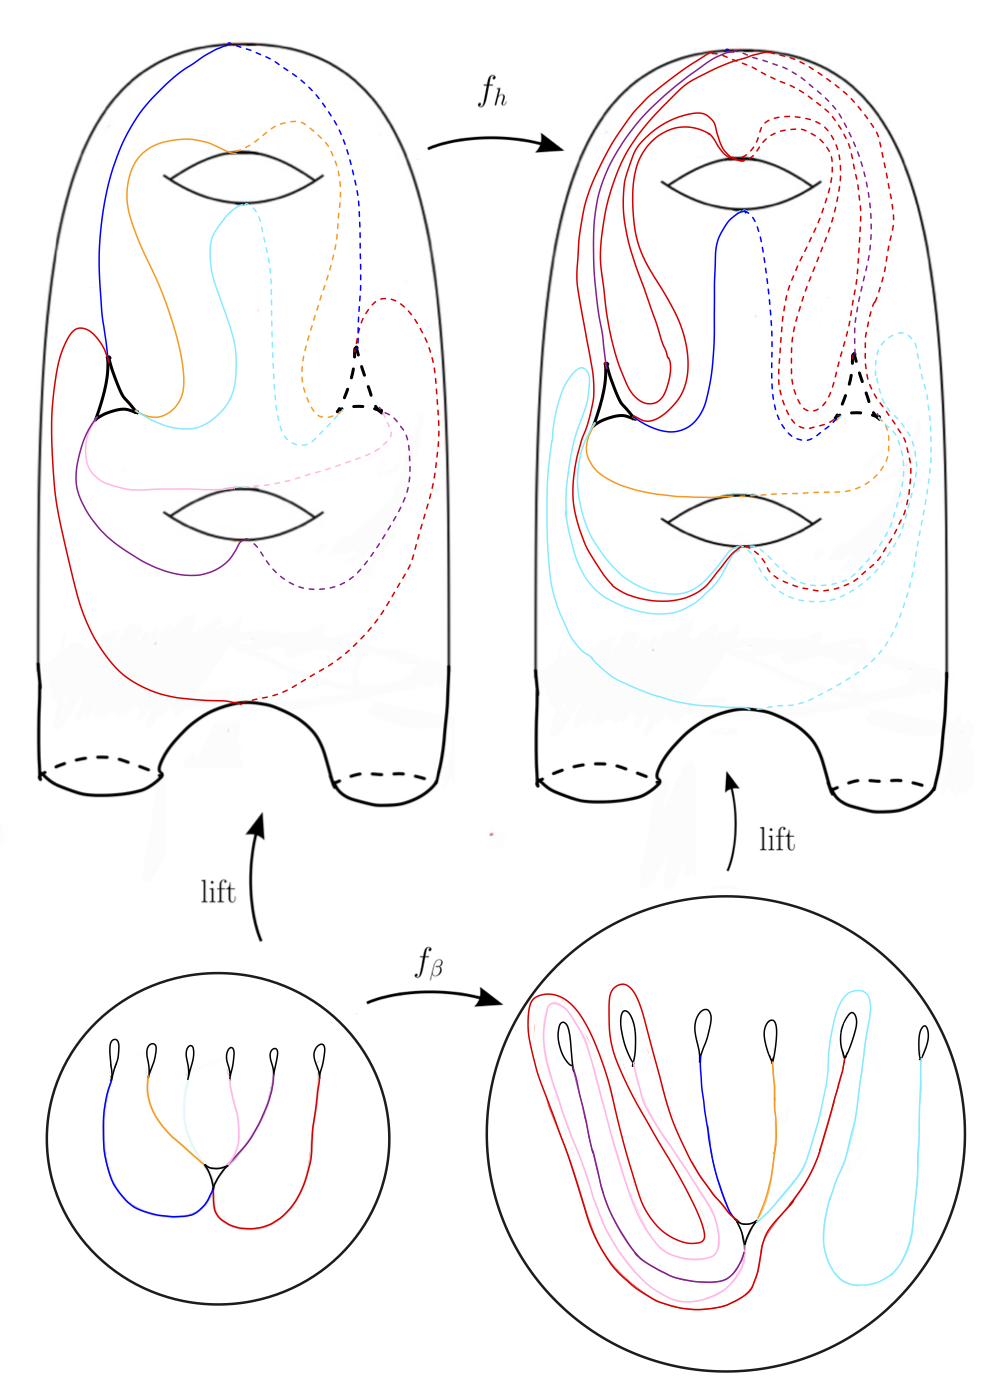
\includegraphics[width=0.8\linewidth]{figures/lifting.png}
    \caption[Visual lift of a train track under the Birman-Hilden correspondence]{Lifting a train track and train track map from $D_6$ to $\Sigma_2^2$. Dashed edges indicate the back side of the surface.}
    \label{fig:reinoso_lift_visual}
\end{figure}

\subsection{Smoothing Infinitesimal Polygons at Branch Points}
A necessary local modification to the lifted train track occurs at the branch points themselves. In a standard track on the disk, a marked point $q_i$ may be surrounded by an infinitesimal $k$-gon (where $k \ge 1$), which represents a $k$-pronged singularity in the invariant foliation. Because the branched covering map $\pi$ behaves locally like the complex map $w = z^2$ at the branch points, the strict topological preimage of this $k$-gon is an infinitesimal $2k$-gon enclosing the lifted Weierstrass point in $\Sigma_2^2$.

While this $2k$-gon correctly captures the doubled cone angle of the lifted foliation, the raw geometric lift retains ``pinched'' internal cusps where the lifted infinitesimal edges meet. To ensure the lifted track efficiently carries the pseudo-Anosov map $\phi_\Phi$ and correctly acts as a $C^1$ smoothing of the unstable foliation, we must apply a local \emph{smoothing} operation to these regions. This operation flattens the inward-pointing cusps, merging the infinitesimal edges into a continuous boundary. We illustrate this in Figure \ref{fig:reinoso_smoothing}, which demonstrates the two distinct geometric outcomes of this operation:

\begin{enumerate}
    \item \textbf{The $k=1$ Case (Top):} If the original marked point was enclosed by a monogon, it lifts to a 2-cusped bigon. In the theory of measured foliations, a 2-pronged singularity is geometrically degenerate; it corresponds merely to a regular, smooth point. Smoothing flattens the two cusps, merging the incident real edges into a single continuous line and entirely deleting the switches associated with the branch point.
    \item \textbf{The $k \ge 2$ Case (Bottom):} If the original marked point was enclosed by a higher-order polygon (e.g., a bigon lifting to a 4-gon, as shown), the $2k$-pronged singularity is retained. The smoothing operation flattens the internal cusps, ``opening up'' the center to form a standard smooth polygonal complementary region with $2k$ sides, accurately bounding the $2k$-pronged saddle.
\end{enumerate}

\begin{figure}[ht]
    \centering
    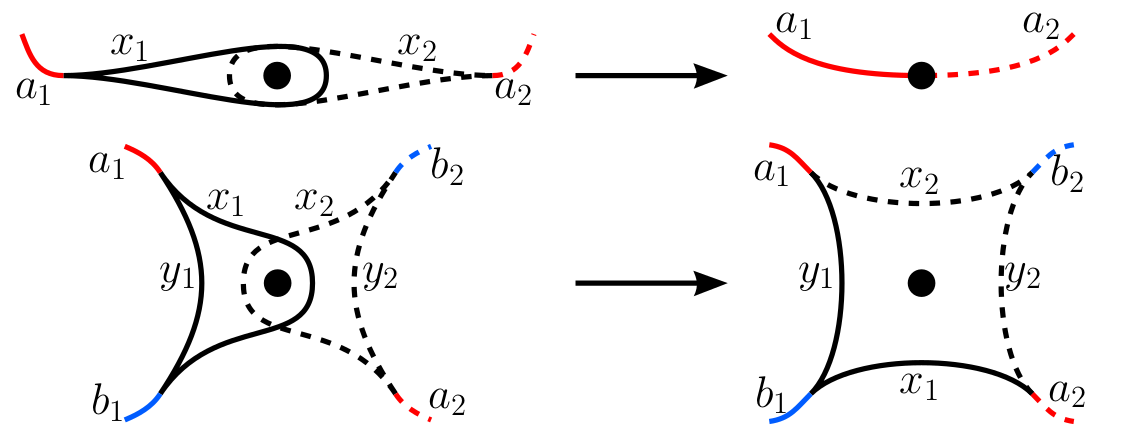
\includegraphics[width=0.8\linewidth]{figures/smoothing.png}
    \caption[Local smoothing of lifted polygons]{The local smoothing operation at branch points. Top: An infinitesimal monogon ($k=1$) lifts to a bigon, which is smoothed into a regular real edge. Bottom: An infinitesimal bigon ($k=2$) at a branch point lifts to a 4-gon with pinched internal cusps, which is smoothed into a proper 4-sided polygonal complementary region. Image courtesy of Braeden Reinoso \cite{reinoso2024pseudo}.}
    \label{fig:reinoso_smoothing}
\end{figure}

\subsection{The Trace Lemma}
Suppose the braid $\beta$ is carried by $\tau$ via the train track map $f_\beta: \tau \to \tau$. While the lifted track $\tilde{\tau}$ is uniquely determined by the geometry described above, the map $f_\beta$ does not lift uniquely. There are exactly two fiber-preserving train track maps
\[
\tilde{f}, \tilde{g} \colon \tilde{\tau} \to \tilde{\tau}
\]
satisfying the covering relation $\pi \circ \tilde{f} = \pi \circ \tilde{g} = f_\beta \circ \pi$. These two lifts are related by the covering involution: $\tilde{g} = \iota \circ \tilde{f}$.

To study the knot monodromy, we must identify the \textbf{canonical lift}. Recall from Proposition \ref{prop:capping off} that the hyperelliptic involution swaps the two fixed points $z$ and $p$, and thus swaps the corresponding boundary components $\partial_z$ and $\partial_p$ of $\Sigma_2^2$. However, the geometric monodromy $\phi_h$ corresponds to a map that fixes the boundary of the knot exterior pointwise. Identifying $\partial_p$ with the boundary of the knot complement, the canonical lift $\tilde{f}_h$ is the unique lift that preserves the component $\partial_p$ (mapping it to itself), whereas the non-canonical lift $\tilde{g}$ swaps $\partial_p$ and $\partial_z$.

A key utility of this construction is the ability to relate the fixed points of the surface homeomorphism $\phi_\Phi$ to the combinatorial properties of the disk map $f_\beta$. In particular, the presence of fixed points for $\phi_\Phi$ can often be detected strictly by the trace of the transition matrix of the disk map. We encapsulate this relationship in the following lemma, which is essential for our detection arguments.

\begin{lemma}[The Trace Lemma, \cite{reinoso2024pseudo}]
\label{lem:trace_lemma}
Let $\beta \in \mathrm{Mod}(D_n)$ be a pseudo-Anosov braid carried by a standard train track $\tau$, and let $f_\beta: \tau \to \tau$ be the induced train track map. Let $\tilde{f}_h$ be the canonical symmetric lift of $\beta$ to the surface $\Sigma_2^2$ (the lift preserving the boundary component $\partial_p$). If the pseudo-Anosov representative $\phi_\Phi$ is fixed-point free (FPF) in the interior of $\Sigma_2^2$, then the trace of the transition matrix $M(f_\beta)$ must be zero.
\end{lemma}
\begin{proof}[Proof Sketch]
The fixed points of $\phi_\Phi$ are contained in the preimage of the fixed points of $\phi_\beta$. For an efficient train track map, fixed points of the map on the graph correspond to fixed points of the homeomorphism (singularities or regular fixed points).

Suppose $\mathrm{tr}(M(f_\beta)) > 0$. Then $f_\beta$ has a fixed point on the interior of some real edge $e \in \tau$. This edge lifts to a pair of edges $e_1, e_2$ in $\tilde{\tau}$ which are swapped by $\iota$. A fixed point $x \in e$ lifts to a pair $\{y, \iota(y)\}$ in $\tilde{\tau}$, and the canonical lift $\tilde{f}_h$ must map this fiber to itself.

The two lifts $\tilde{f}_h$ and $\iota \circ \tilde{f}_h$ act differently on this fiber: one fixes each point individually, while the other swaps them. The canonical lift $\tilde{f}_h$ is distinguished by the requirement that it preserves the boundary component $\partial_p$, while $\iota \circ \tilde{f}_h$ swaps $\partial_p$ and $\partial_z$. Tracking the boundary-preserving condition through the local geometry near $x$ (specifically, comparing the orientations of the lifted real edges at the boundary), one finds that the canonical lift $\tilde{f}_h$ fixes each point of the fiber $\{y, \iota(y)\}$ individually rather than swapping them. Consequently, both $y$ and $\iota(y)$ are fixed points of $\tilde{f}_h$, and they correspond to fixed points of the geometric representative $\phi_\Phi$ in the interior of $\Sigma_2^2$.

Thus, if the trace is non-zero, $\phi_\Phi$ retains an interior fixed point, contradicting the FPF hypothesis. The vanishing of the trace is therefore necessary for $\phi_\Phi$ to be FPF.
\end{proof}

We will use the Trace Lemma to rule out pseudo-Anosov candidates for the monodromy of our knot. Because Heegaard Floer homology constraints imply that our hypothetical knot must have exactly one fixed point corresponding to the original un-capped surface (which we factored out into the boundary of $\Sigma_2^2$), we can immediately eliminate any braid $\beta$ for which $M(f_\beta)$ has non-zero trace.